% Figure 1. The estimate, the two bootstraps, and the three results.
% Two samples feed one formula. The production sample has judge labels only and gives q-hat.
% The validation sample has human and judge labels and gives sensitivity a-hat and
% specificity b-hat. The corrected pass rate is the Rogan-Gladen ratio. A bootstrap repeats
% the calculation on resampled data. The validation-only bootstrap resamples the validation
% sample only; the two-sample bootstrap resamples both. Badges 1 to 3 mark where each
% result enters. The cells are schematic: the letter is the judge's label.
% Every result number comes from fig1-numbers.tex, which make_figures.py writes from the
% CSV files in results/.
% Build: python3 make_figures.py (needs pdflatex with TikZ, and pdftocairo).
% Size: drawn at 162 mm with 7 pt words, then scaled to the 203 mm width of Figures 2 to 4.
\documentclass[border=0pt]{standalone}
\pdfinfoomitdate=1
\pdftrailerid{}
\usepackage{helvet}
\renewcommand{\familydefault}{\sfdefault}
\usepackage{amsmath}
\usepackage{graphicx}
\usepackage{tikz}
\usetikzlibrary{arrows.meta,calc,fit}

\definecolor{neutral}{HTML}{F1F5F9}
\definecolor{neutralline}{HTML}{62748E}
\definecolor{ink}{HTML}{172B3A}
\definecolor{muted}{HTML}{45556C}
% The colour roles of Figures 2 to 4: orange for the validation-only bootstrap, blue for the
% two-sample bootstrap.
\definecolor{validationonly}{HTML}{FFEDD4}
\definecolor{validationonlyline}{HTML}{F54900}
\definecolor{twosample}{HTML}{DFF2FE}
\definecolor{twosampleline}{HTML}{0084D1}

% Written by make_figures.py from the CSV files in results/. Do not edit.
\def\OnlyCoverage{82.1}
\def\TwoSampleCoverage{94.2}
\def\ProductionCases{268}
\def\ValidationLabels{200}
\def\NoInterval{13.4}
\def\Discarded{12.0}
\def\WeakJ{0.20}
\def\WeakLabels{40}
\def\DriftBias{5.2}
\def\DriftCoverage{70.5}
\def\DriftFall{5}


\newcommand{\seven}{\fontsize{7}{8.5}\selectfont}
\newcommand{\nine}{\fontsize{9}{11}\selectfont}

\tikzset{
  every node/.append style={text=ink, font=\seven},
  stage/.style={draw=neutralline, fill=neutral, line width=0.6pt, rounded corners=3pt},
  card/.style={draw=neutralline, fill=white, line width=0.6pt, rounded corners=3pt},
  title/.style={font=\seven\bfseries, inner sep=1pt},
  sym/.style={inner sep=1pt},
  word/.style={text=muted, inner sep=1pt},
  headline/.style={font=\nine\bfseries, inner sep=1pt},
  tag/.style={line width=0.6pt, rounded corners=2pt, inner xsep=3pt, inner ysep=2pt,
    minimum height=4.2mm},
  validationonlytag/.style={tag, draw=validationonlyline, fill=validationonly},
  twosampletag/.style={tag, draw=twosampleline, fill=twosample},
  badge/.style={circle, fill=ink, text=white, font=\seven\bfseries, inner sep=0pt,
    minimum size=3.6mm},
  cell/.style={rectangle, rounded corners=1pt, inner sep=0pt, minimum width=3.7mm,
    minimum height=3.5mm, line width=0.5pt, draw=neutralline},
  passcell/.style={cell, fill=white},
  failcell/.style={cell, fill=neutralline!38},
  flow/.style={-{Stealth[length=2.4mm, width=2mm]}, line width=1.2pt, draw=ink,
    shorten >=1.5pt, rounded corners=3pt},
  assumed/.style={{Stealth[length=2mm, width=1.7mm]}-{Stealth[length=2mm, width=1.7mm]},
    line width=0.8pt, draw=ink, dash pattern=on 3pt off 2pt},
}

% A row of cells: #1 the x of the first centre, #2 the y, #3 the judge labels.
\def\step{0.44}
\newcommand{\cells}[3]{%
  \foreach \l [count=\i] in {#3} {%
    \if\l P\node[passcell] at ({#1 + \step*(\i - 1)}, #2) {P};%
    \else\node[failcell] at ({#1 + \step*(\i - 1)}, #2) {F};\fi}}

\begin{document}
\scalebox{1.255}{%
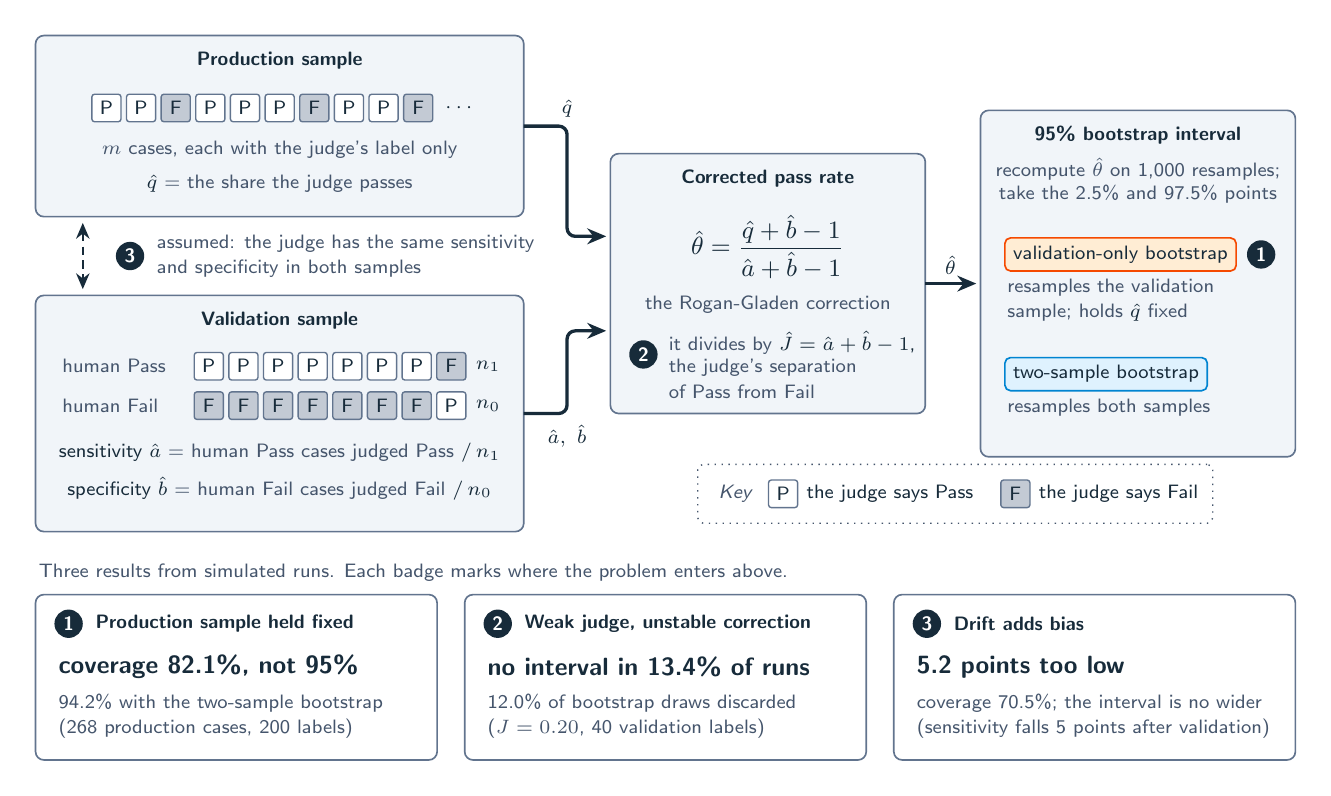
\begin{tikzpicture}
\useasboundingbox (-0.1,0.1) rectangle (16.1,-9.3);
\fill[white] (-0.1,0.1) rectangle (16.1,-9.3);

% ================================================================ the production sample
\draw[stage] (0,0) rectangle (6.2,-2.3);
\node[title] at (3.1,-0.32) {Production sample};
\cells{0.9}{-0.92}{P,P,F,P,P,P,F,P,P,F}
\node[sym] at (5.4,-0.92) {$\cdots$};
\node[word] at (3.1,-1.45) {$m$ cases, each with the judge's label only};
\node[sym] at (3.1,-1.88) {$\hat q$ \textcolor{muted}{= the share the judge passes}};

% ================================================================ the shared assumption
\draw[assumed] (0.6,-2.38) -- (0.6,-3.22);
\node[badge] at (1.2,-2.8) {3};
\node[word, anchor=west] at (1.5,-2.64) {assumed: the judge has the same sensitivity};
\node[word, anchor=west] at (1.5,-2.96) {and specificity in both samples};

% ================================================================ the validation sample
\draw[stage] (0,-3.3) rectangle (6.2,-6.3);
\node[title] at (3.1,-3.62) {Validation sample};
\node[word, anchor=west] at (0.3,-4.2) {human Pass};
\cells{2.2}{-4.2}{P,P,P,P,P,P,P,F}
\node[sym, anchor=west] at (5.55,-4.2) {$n_1$};
\node[word, anchor=west] at (0.3,-4.7) {human Fail};
\cells{2.2}{-4.7}{F,F,F,F,F,F,F,P}
\node[sym, anchor=west] at (5.55,-4.7) {$n_0$};
\node[sym] at (3.1,-5.3) {sensitivity $\hat a$ \textcolor{muted}{= human Pass cases
  judged Pass} $/\,n_1$};
\node[sym] at (3.1,-5.75) {specificity $\hat b$ \textcolor{muted}{= human Fail cases
  judged Fail} $/\,n_0$};

% ================================================================ the corrected pass rate
\draw[stage] (7.3,-1.5) rectangle (11.3,-4.8);
\node[title] at (9.3,-1.82) {Corrected pass rate};
\node[font=\nine] at (9.3,-2.68) {$\hat\theta = \dfrac{\hat q + \hat b - 1}{\hat a + \hat b - 1}$};
\node[word] at (9.3,-3.42) {the Rogan-Gladen correction};
\node[badge] at (7.72,-4.05) {2};
\node[sym, anchor=west] at (8.0,-3.9) {\textcolor{muted}{it divides by} $\hat J = \hat a + \hat b - 1$,};
\node[word, anchor=west] at (8.0,-4.22) {the judge's separation};
\node[word, anchor=west] at (8.0,-4.52) {of Pass from Fail};

% ================================================================ the bootstrap interval
\draw[stage] (12.0,-0.95) rectangle (16.0,-5.35);
\node[title] at (14.0,-1.27) {95\% bootstrap interval};
\node[word] at (14.0,-1.7) {recompute $\hat\theta$ on 1,000 resamples;};
\node[word] at (14.0,-2.02) {take the 2.5\% and 97.5\% points};
\node[validationonlytag, anchor=west] (onlytag) at (12.3,-2.78) {validation-only bootstrap};
\node[badge, anchor=west] at ($(onlytag.east) + (0.12,0)$) {1};
\node[word, anchor=west] at (12.3,-3.2) {resamples the validation};
\node[sym, anchor=west] at (12.3,-3.52) {\textcolor{muted}{sample; holds} $\hat q$ \textcolor{muted}{fixed}};
\node[twosampletag, anchor=west] at (12.3,-4.3) {two-sample bootstrap};
\node[word, anchor=west] at (12.3,-4.72) {resamples both samples};

% ---------------------------------------------------------------- the flow
\draw[flow] (6.2,-1.15) -- (6.75,-1.15) -- (6.75,-2.55) -- (7.3,-2.55);
\node[sym, anchor=south] at (6.75,-1.08) {$\hat q$};
\draw[flow] (6.2,-4.8) -- (6.75,-4.8) -- (6.75,-3.75) -- (7.3,-3.75);
\node[sym, anchor=north] at (6.75,-4.9) {$\hat a,\ \hat b$};
\draw[flow] (11.3,-3.15) -- (12.0,-3.15);
\node[sym, anchor=south] at (11.62,-3.08) {$\hat\theta$};

% ---------------------------------------------------------------- the key
\node[font=\seven\itshape, text=muted, anchor=west] (keylabel) at (8.55,-5.82) {Key};
\node[passcell, anchor=west] (keypass) at (9.3,-5.82) {P};
\node[sym, anchor=west] (keypassw) at (9.75,-5.82) {the judge says Pass};
\node[failcell, anchor=west] (keyfail) at (12.25,-5.82) {F};
\node[sym, anchor=west] (keyfailw) at (12.7,-5.82) {the judge says Fail};
\node[draw=muted, dotted, line width=0.5pt, rounded corners=2pt, inner sep=4pt,
  fit=(keylabel)(keypass)(keypassw)(keyfail)(keyfailw)] {};

% ================================================================ the three results
\node[word, anchor=west] at (0,-6.82) {Three results from simulated runs. Each badge
  marks where the problem enters above.};

\draw[card] (0,-7.1) rectangle (5.1,-9.2);
\node[badge] at (0.42,-7.47) {1};
\node[title, anchor=west] at (0.72,-7.47) {Production sample held fixed};
\node[headline, anchor=west] at (0.25,-8.02) {coverage \OnlyCoverage\%, not 95\%};
\node[word, anchor=west] at (0.25,-8.48) {\TwoSampleCoverage\% with the two-sample bootstrap};
\node[word, anchor=west] at (0.25,-8.8) {(\ProductionCases{} production cases, \ValidationLabels{} labels)};

\draw[card] (5.45,-7.1) rectangle (10.55,-9.2);
\node[badge] at (5.87,-7.47) {2};
\node[title, anchor=west] at (6.17,-7.47) {Weak judge, unstable correction};
\node[headline, anchor=west] at (5.7,-8.02) {no interval in \NoInterval\% of runs};
\node[word, anchor=west] at (5.7,-8.48) {\Discarded\% of bootstrap draws discarded};
\node[word, anchor=west] at (5.7,-8.8) {($J = \WeakJ$, \WeakLabels{} validation labels)};

\draw[card] (10.9,-7.1) rectangle (16.0,-9.2);
\node[badge] at (11.32,-7.47) {3};
\node[title, anchor=west] at (11.62,-7.47) {Drift adds bias};
\node[headline, anchor=west] at (11.15,-8.02) {\DriftBias{} points too low};
\node[word, anchor=west] at (11.15,-8.48) {coverage \DriftCoverage\%; the interval is no wider};
\node[word, anchor=west] at (11.15,-8.8) {(sensitivity falls \DriftFall{} points after validation)};

\end{tikzpicture}}
\end{document}
